%------------------------------------------------------------------------
%Editar Diplomado
\hypertarget{cv:GestionarModulos}{\section{Gestionar Módulos}} \label{sec:GestionarModulos}

	Esta funcionalidad le permitirá las acciones necesarias para controlar los módulos y visualizarlos en una tabla en el proyecto sobre el que se está operando y solicitar el registro de uno nuevo.

		\subsection{Procedimiento}

			%Pasos de procedimiento
			\begin{enumerate}
				
			\item Ingrese a un proyecto existente desde la pantalla \ref{fig:GestionarProyectosColaborador}.
	
			\item Seleccione la opción \textbf{Modulos} del menú \ref{fig:MN-LPC}.
	
			\item Se mostrará la pantalla \ref{fig:GestionarModulos} ''Gestionar Módulos''.

			%Pantalla
			\begin{figure}[htbp!]
				\begin{center}
					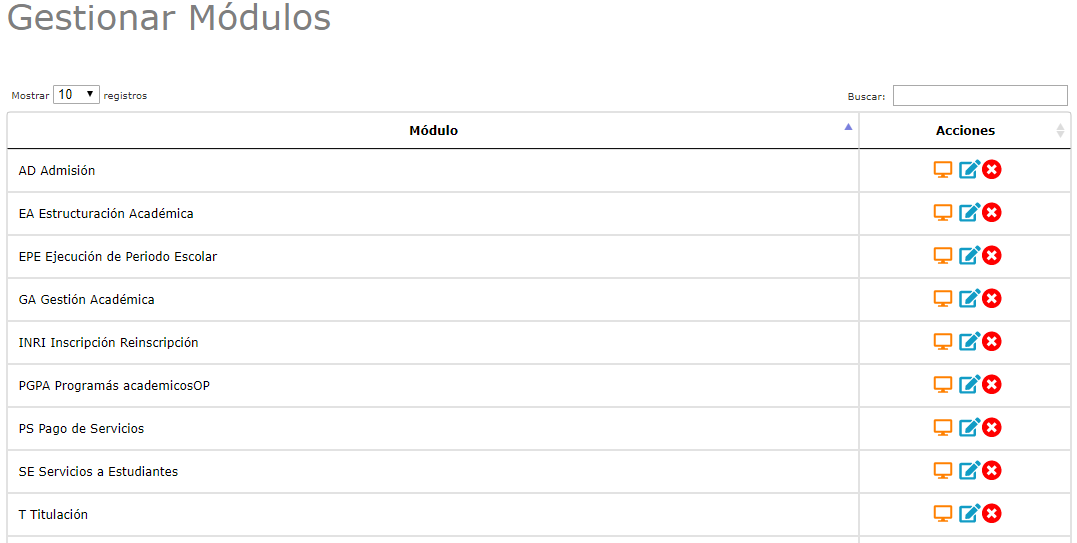
\includegraphics[scale=0.6]{roles/lider/modulos/pantallas/IU5gestionarModulos}
					\caption{Gestionar Módulos}
					\label{fig:GestionarModulos}
				\end{center}
			\end{figure}
		
				\item Seleccione la operación que desea realizar:
			
			Para (\hyperlink{cv:registrarModulo}{Registrar}) dé clic en el botón \IURegistrar.
			
			Para (\hyperlink{cv:modificarModulo}{Modificar}) dé clic en el icono \IUEditar{} de algún proyecto ya registrado.
			
			Para (\hyperlink{cv:eliminarProyecto}{Eliminar}) dé clic en el icono \IUBotonEliminar{} de algún proyecto ya registrado.
			
			
			\end{enumerate}